\documentclass[12pt]{article}
\usepackage[utf8]{inputenc}
\usepackage{natbib}
\usepackage{url}
\usepackage{graphicx}
\title{The Impact of Shifting Prey Availability on Atlantic Puffin (\textit{Fratercula arctica}) Chick Provisioning and Breeding Success}
\author{Nora Losch}
\date{\today}


\begin{document}

\maketitle



The Atlantic Puffin (\textit{Fratercula arctica}) is one of the most recognizable seabirds of the North Atlantic, but its populations are under increasing threat. As a specialist predator that feeds primarily on small forage fish, the puffin acts as a sensitive indicator species, or "sentinel," reflecting the health of the surrounding marine ecosystem. In recent decades, rapid ocean warming attributed to climate change has begun to trigger significant shifts in these ecosystems, posing a direct threat to puffin survival \ref{fig:placeholder}.

The core of the issue lies in the puffin's reliance on specific, high-energy prey to successfully raise a chick. Puffins are "central-place foragers" during the breeding season, meaning they must commute from their nesting burrow to foraging grounds and back. Their reproductive success is therefore highly dependent on the availability of nutrient-rich fish, such as sand eels (\textit{Ammodytes marinus}) and juvenile herring (\textit{Clupea harengus}), within a viable flight range of the colony.

However, these cold-water fish species are themselves highly sensitive to rising sea surface temperatures. Warmer waters are causing shifts in prey distribution, forcing fish populations to move deeper or further north into cooler waters \citep{frederiksen2007role}. This creates a "spatial mismatch" for the puffins. While adult birds may be able to survive by expending more energy to fly further, the "provisioning cost" to the chick becomes unsustainable. Adults may return to the nest with fewer fish, fish of lower nutritional quality, or so infrequently that the chick starves or develops too slowly to fledge—a phenomenon known as "trophic mismatch".

This study will investigate the direct consequences of this climate-induced foraging challenge. By comparing recent data on adult foraging trip durations, diet composition, and chick growth rates with historical colony data and local sea surface temperature anomalies, this research aims to quantify the threshold at which shifting prey availability leads to critical failures in puffin breeding success. Understanding this mechanism is vital for predicting population trajectories and identifying potential climate refugia for this vulnerable species \citep{jessopp2013transatlantic}.


\begin{figure}
    \centering
    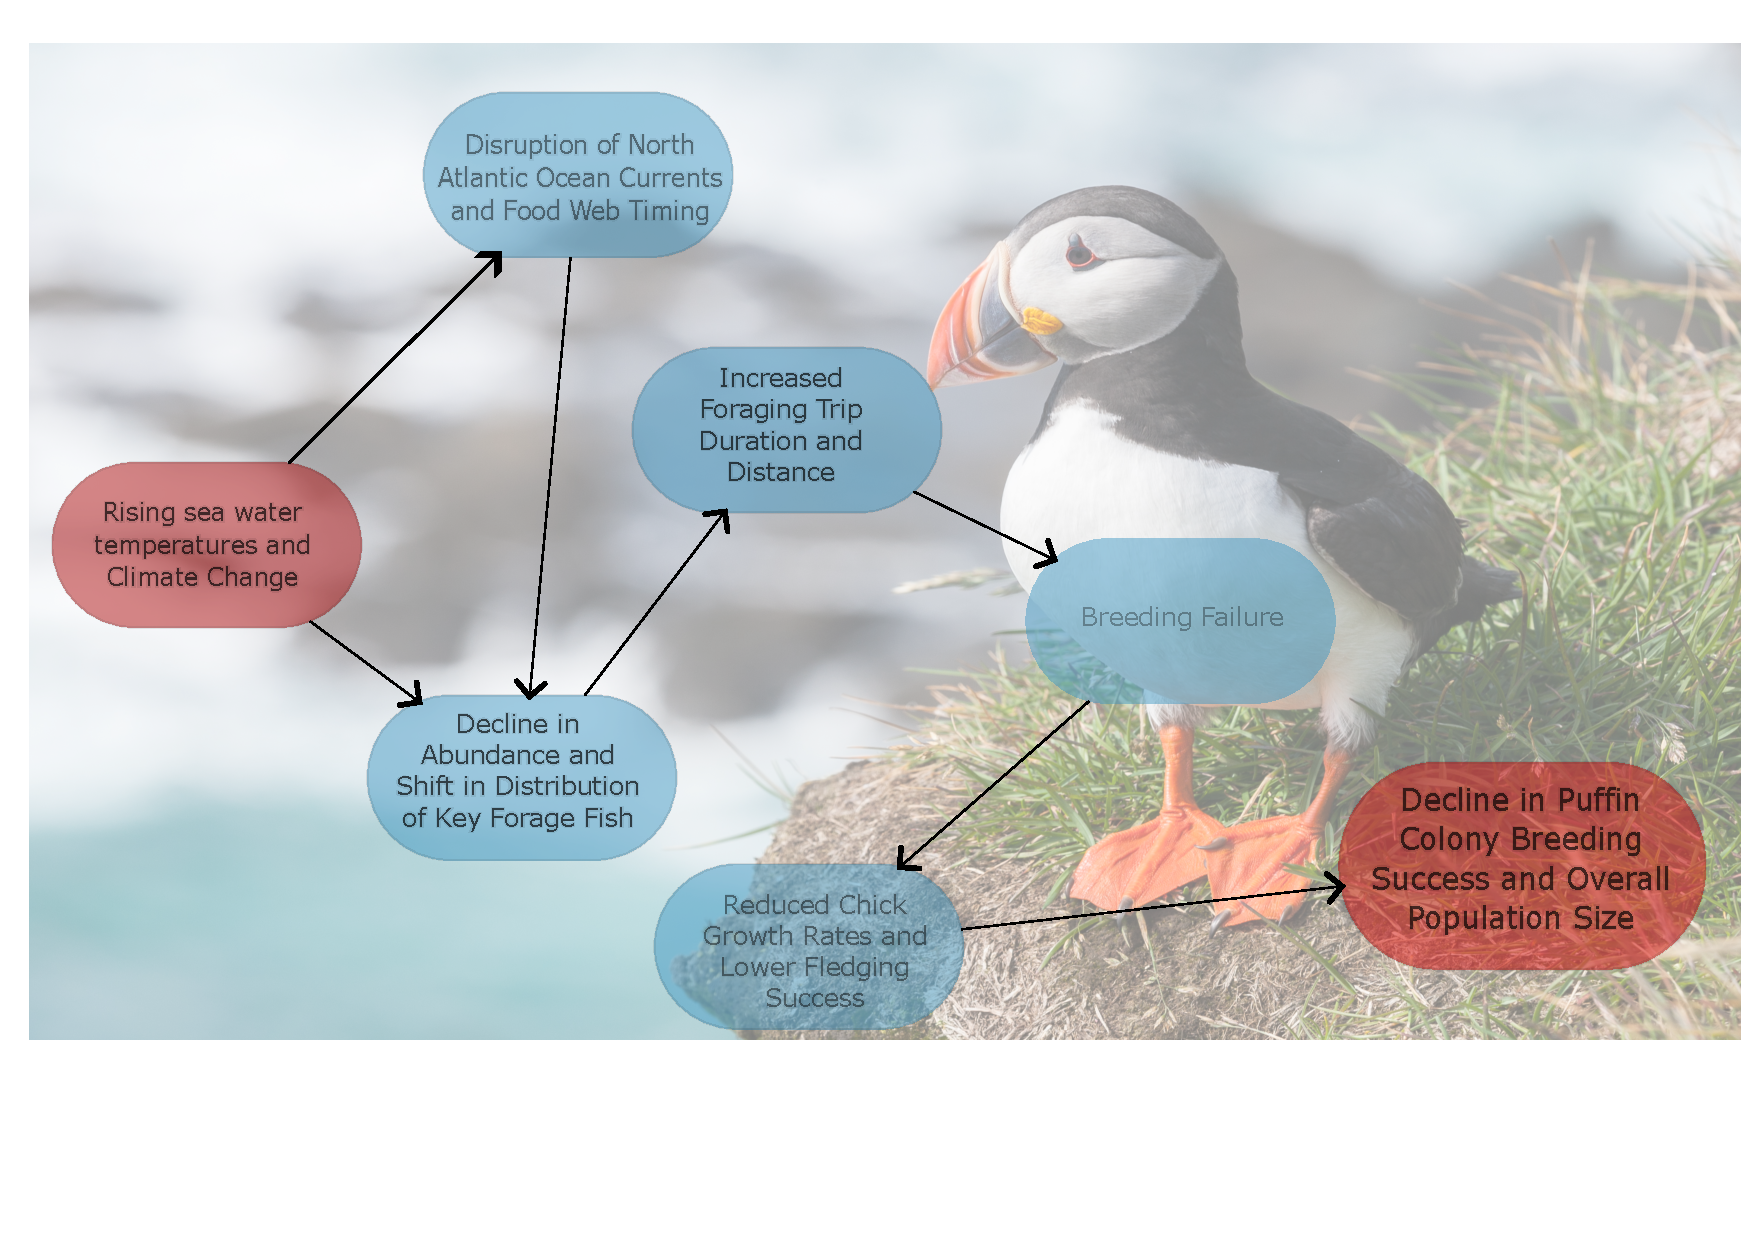
\includegraphics[width=1\linewidth]{puffin.png}
    \caption{This chart represents the primary hypothesized mechanism driving the decline in puffin breeding success.}
    \label{fig:placeholder}
\end{figure}

\bibliographystyle{plainnat}
\bibliography{references}


\end{document}